% using aastex version 6.2
\documentclass[twocolumn,fleqn]{aastex62}
\usepackage{amsmath}
\usepackage{microtype}
\usepackage{bm}
\usepackage{dsfont}
\usepackage{listings}
\usepackage{url}
\usepackage{tikz}
\usetikzlibrary{shapes,arrows}
\usepackage{natbib}
\usepackage{booktabs}
\lstset{
	basicstyle=\ttfamily,
	mathescape,
}

%%  twocolumn   : two text columns, 10 point font, single spaced article.
%%                This is the most compact and represent the final published
%%                derived PDF copy of the accepted manuscript from the publisher
%%  manuscript  : one text column, 12 point font, double spaced article.
%%  preprint    : one text column, 12 point font, single spaced article.  
%%  preprint2   : two text columns, 12 point font, single spaced article.
%%  modern      : a stylish, single text column, 12 point font, article with
%% 		  wider left and right margins. This uses the Daniel
%% 		  Foreman-Mackey and David Hogg design.
%%  RNAAS       : Preferred style for Research Notes which are by design 
%%                lacking an abstract and brief. DO NOT use \begin{abstract}
%%                and \end{abstract} with this style.

%%  astrosymb    : Loads Astrosymb font and define \astrocommands. 
%%  tighten      : Makes baselineskip slightly smaller, only works with 
%%                 the twocolumn substyle.
%%  times        : uses times font instead of the default
%%  linenumbers  : turn on lineno package.
%%  trackchanges : required to see the revision mark up and print its output
%%  longauthor   : Do not use the more compressed footnote style (default) for 
%%                 the author/collaboration/affiliations. Instead print all
%%                 affiliation information after each name. Creates a much
%%                 long author list but may be desirable for short author papers
%% \documentclass[twocolumn,linenumbers,trackchanges]{aastex62}

\newcommand{\vdag}{(v)^\dagger}
\newcommand\aastex{AAS\TeX}
\newcommand\latex{La\TeX}
\newcommand{\thickbar}[1]{\mathbf{\bar{\text{$#1$}}}}

\graphicspath{{./}{figures/}}
\shorttitle{PACO in Pynpoint}
\shortauthors{Nasedkin}

%\tikzstyle{block} = [rectangle, draw, fill=white, text width=5em, text centered,  minimum height=2em]
%\tikzstyle{line} = [draw, -latex']
\begin{document}
	
	
	\title{Implementing the PACO Algorithm as a Pynpoint Module.}
	
	
	\correspondingauthor{Evert Nasedkin}
	\email{evertn@student.ethz.ch}
	
	\author{Evert Nasedkin}
	\affil{ETH Z\"{u}rich, Exoplanets and Habitability Group}
	\author{Polychronis Patapis}
	\affil{ETH Z\"{u}rich, Exoplanets and Habitability Group}

\setlength{\mathindent}{10pt}
\begin{abstract}
lorum ipsum stuff stuff stuff

blah
b

blah
\end{abstract}

\section{Introduction}
% Standard boilerplate about HCI
The field of exoplanet astronomy has seen dramatic growth since the initial discovery from \cite{ref:quel} in 19??. 
With the advent of high-contrast imaging techniques in ???? CITE, we have been able to observe exoplanets in regimes inaccessible through other detection methods.
Through the combination of dedicated instrumentation CITE(NaCo,Sphere,GPI), adaptive optics CITE and data processing techniques, we have been able to observe around 12,13? companions as of 2019, with the hope for many more discoveries following the completion of next generation observatories such as JWST and the ELT. 

This report focuses on the implementation and testing of the Patch Covariance, or PACO algorithm for point source detection. PACO looks for spatio-temporal correlations in data taking in ADI mode, and offers a statistical interpretation of the detection maps.
\subsection{ADI}
% Include nice figure showing ADI
\begin{figure}[h]
	%\includegraphics[width=\linewidth]{}
	\caption{\label{fig:adi} Outline of standard angular differential imaging processing.}
\end{figure}
\section{PACO Statistical Model}
% Figure from PACO paper showing columns
There are two primary implementations of the PACO algorithm, based.
First we will consider the full implementation, followed by the assumptions made to create the second fast algorithm.
We will also discuss the addition of PACO to the Pynpoint analysis package.

The Patch Covariance, or PACO algorithm works by considering the known trajectory of a companion through an image stack taken with a pupil-stabilized telescope. 
It is important to note that while the companion will follow an arc through the image stack, speckle noise from the telescope will remain stationary. 
This allows us to distinguish the weak source from the much stronger background noise.
The following section will closely follow the presentation of \cite{PACO}, with some changes to notation to aid with clarity. 

\begin{figure}[h]
	\centering
	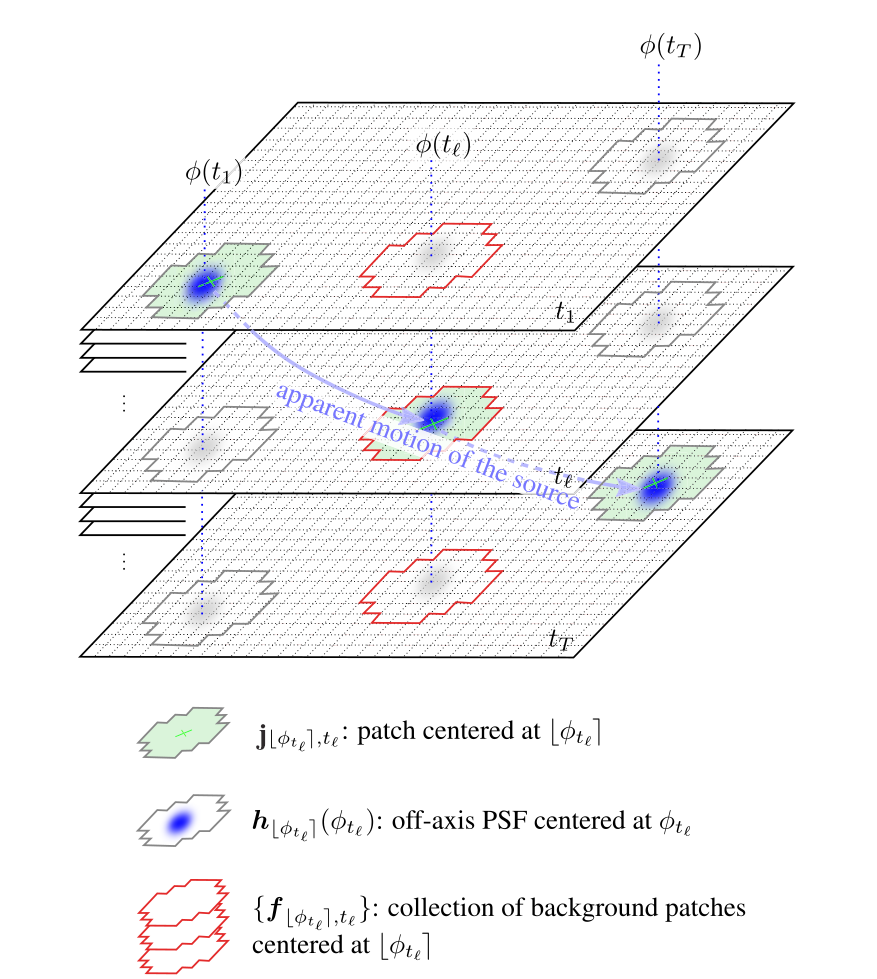
\includegraphics[width=\linewidth]{figures/PacoVis.png}
	\caption{\label{fig:patches} Patches are selected from each temporal frame based on the hypothesis that a signal was located at an initial pixel, and follows a rotation through the parallactic angle through the frames.}
\end{figure}
\begin{table}
	\centering
	\begin{tabular}{rl}
		\toprule
		Symbol & Description\\
		\midrule
		M & Number of frames\\
		N & Number of pixels per frame\\
		K & Number of pixels per patch\\
		\midrule
		$\theta$ & 2D Pixel location\\
		$\phi_{t}$ & Angular sub-pixel location in frame t\\
		$[\phi_{t}]$ & Angular location to nearest pixel\\
		\midrule
		$j$ & Intensity at a point \\
		$f$ & Intensity due to background at a point\\
		$\alpha$ & Flux of a source at a specified location\\
		$\mathbf{h}$ & 2D PSF template\\
		\bottomrule		
	\end{tabular}
	\caption{\label{tab:notes}Summary of PACO notation.}
\end{table}
Consider a stack of M temporal frames, where each frame contains N pixels. 
We will be considering the hypothesis, $\mathcal{H}_{1}$, that there is a planet located at the position of a given pixel to the background only hypothesis  $\mathcal{H}_{0}$. 
This comparison can be formalized as a likelihood ratio test.

We use the additional knowledge about the trajectory of the planet position through the image stack to determine whether there is a signal when compared to the background only. 
For a given initial angular position $\phi_{0}$, this trajectory is a rotation through each temporal frame, which we write as $\mathcal{F}_{t}(\phi_{0})$. The index $t$ runs from 0 to M frames.

For $\mathcal{H}_{1}$, the observed intensity $j$ at a given location $\theta$ will be the sum of the background intensity $f$, together with some intensity from the source. 
We will use square brackets $[\theta]$ to denote a pixel-centered location, as opposed to a true 2D coordinate $\theta$.
Also note that $[\theta]$ will be indexed per pixel as $[\theta]_{n}$ if necessary.
For a single frame, the source is modeled as a template PSF $\textbf{h}$ multiplied by source flux $\alpha$, centered on the pixel $[\theta]$. Considering the PSF template at only at the location $\theta$, we write the total intensity at that point as:
\begin{equation}\label{eqn:frame}
j(\theta) = \alpha h(\theta) + f(\theta)
\end{equation}
Both the template PSF and the background vary with time, and we generalize Eqn. \ref{eqn:frame} using the 2D angular location at time t, denoted as $\phi_{t} = \mathcal{F}(\phi_{0})$. 
As above, the closest on grid location will be notated with square brackets.
\begin{equation}
j(\theta,\phi_{t}) = \alpha h(\theta,\phi_{t}) + f(\theta,t)
\end{equation}
We restrict $\alpha$ to be positive, and 0 in the absence of a source.
As companions are relatively rare, we do not consider the case where two sources can overlap.
If the background noise is distributed according to some PDF $p_{f}$, each observation can be treated as a random draw from this distribution, with a source of strength $\alpha$ overlaid. 
Thus the joint probability of drawing a particular collection of intensities $\{j(\theta_{k},t)\}$ at a locations $[\theta]_{k=0:N}$ and times $t=0:M$ with a source of flux $\alpha$ can be written as:
\begin{equation}
p_{j}(\{j\}|\alpha,\phi_{t}) = p_{f}(\{j - \alpha h(\theta,\phi)\})
\end{equation}  
For each possible initial angular position $\phi_{0}$, we can now construct an unbiased maximum likelihood estimator for the flux. 
\begin{equation}
\hat{\alpha} = \textrm{argmax}\left(p_{f}(\{j - \alpha h(\theta,\phi_{0})\})\right)
\end{equation}
With this estimator, we can now construct the hypothesis test, choosing some threshold for detection, again with sets covering the collection of temporal frames $t=0:M$ and pixels $[\theta]_{k=0:N}$.
\begin{align}
\mathcal{H}_{0} &: {j} = \{f\}\\
\mathcal{H}_{1} &: {j} = \alpha \{h(\theta,\phi)\} + \{f\}
\end{align}
Thus we are comparing the null hypothesis that the collection of M observations for each of the N pixels consists of only background fluctuations according to its PDF $f(\theta,\phi)$ to the alternative hypothesis $\mathcal{H}_{1}$ that a source of flux $\alpha$ and PSF $h(\theta,\phi)$ is overlaid on top of the same background. 
By substituting the estimator $\hat{\alpha}$ in place of the true flux $\alpha$, we can write the generalized likelihood ratio test with threshold $\eta$ as:
\begin{equation}\label{eqn:ll}
\log\frac{p_{f}(\{j - \hat{\alpha} h(\theta,\phi)\})}{p_{f}(\{j\})} \gtrless \eta
\end{equation}

\begin{figure}[h]
	\centering
	%\includegraphics[width=\linewidth]{}
	\caption{\label{fig:patch} Patch shapes and sizes}
\end{figure}

To determine the background distribution, a 2D neighbourhood centered around each $\theta$ is chosen.
This \textit{patch} of pixels should be large enough to contain the core of the off axis PSF, and additionally contains the relevant background pixels for the specified location.  
While in general the shape of the patch is arbitrary, a 2D discrete disk is used in this work.
Each temporal slice is considered to be an independent sample, and the number of counts per pixel is large enough to model Poisson counting statistics as normal distributions.
This approximation allows us to write the background distribution in closed-form.
This allows us to write the background distribution for the a patch $\mathbf{j}$ with the collection of backgrounds $\{\mathbf{f}\}_{t=0:M}$ as the product of multivariate normal distributions, defined over each patch that would contain an companion, following the trajectory of $\phi_{t}$:
\begin{equation}\label{eqn:mvg}
p_{f}\left(\{\mathbf{f}([\phi]_{t})\}_{t=0:M}\right) = \prod_{t = 0}^{M}\mathcal{N}\left(\mathbf{f}([\phi]_{t},t),\mathbf{m}([\phi]_{t}),\mathbf{C}([\phi]_{t})\right)
\end{equation}
Where $\mathcal{N}\left(\cdot,\mathbf{m}([\phi]_{t}),\mathbf{C}([\phi]_{t})\right)$ is athe probability density of the multivariate normal distribution with mean $\mathbf{m}$ and covariance $\mathbf{C}$ centered at pixel $[\phi_{t}]$.
To determine the mean and covariance of this distribution, we consider the collection of patches centered on the same pixel $[\theta]$ without following the trajectory to find estimators for the sample mean and covariance.
The sample mean is simply:
\begin{equation}
\hat{\mathbf{m}}([\theta]) = \frac{1}{M}\sum_{t=0}^{M}\mathbf{j}([\theta],t)
\end{equation}

The estimator for the covariance must be regularized to account for the case where the covariance is rank deficient, i.e. when the number of frames is smaller than the number of pixels K in a patch.
A shrinkage approach was used in \cite{}, based on \cite{}, and this approach was used in our implementation.
In short, the estimator for the covariance is written as a combination of the estimator of the sample covariance plus the diagonal of the sample covariance weighted by a shrinkage factor $\hat{\rho}$:

\begin{equation}
\hat{\mathbf{C}} = (1-\hat{\rho})\hat{\mathbf{S}} + \hat{\rho}\hat{\mathbf{F}}
\end{equation}

The estimators $\hat{\mathbf{S}}$ and $\hat{\mathbf{F}}$ are chosen such that one is biased but has small variance, while the other has large variance but minimal bias. 
The parameter $\hat{\rho}$ is chosen to optimize this trade off, and a full derivation can be found in \cite{}.
Each term can be computed as:
\begin{equation}
\hat{\mathbf{S}}(\theta) = \frac{1}{M}\sum_{t = 0}^{M}\left( \mathbf{j}(\theta,t) - \hat{\mathbf{m}}(\theta)\right) \cdot\left( \mathbf{j}(\theta,t) - \hat{\mathbf{m}}(\theta)\right)^{t}
\end{equation}
\begin{equation}
\left[\hat{\mathbf{F}}(\theta)\right]_{ii} = \frac{1}{M}\sum_{t = 0}^{M}\left[ \mathbf{j}(\theta,t) - \hat{\mathbf{m}}(\theta)\right]^{2}_{ii} = \left[\hat{\mathbf{S}}(\theta)\right]_{ii}
\end{equation}
\begin{equation}
\hat{\rho}\left(\hat{\mathbf{S}}(\theta)\right) = \frac{\textrm{tr}\left(\hat{\mathbf{S}}^{2}(\theta)\right) +
\textrm{tr}^{2}\left(\hat{\mathbf{S}}(\theta)\right) -
2\sum_{i=1}^{K}\left[\hat{\mathbf{S}}(\theta)\right]^{2}_{ii}}{(M+1)\left(\textrm{tr}\left(\hat{\mathbf{S}}^{2}(\theta)\right)\right) -
\sum_{i=1}^{K}\left[\hat{\mathbf{S}}(\theta)\right]^{2}_{ii}}
\end{equation}


\subsection{Flux Estimation}
From the multivariate Gaussian model of the background in Eqn. \ref{eqn:mvg} we find that the maximum likelihood estimator for the flux at a given location can be written as:
\begin{equation}
\hat{\alpha} = \frac{\sum_{t = 0}^{M}b_{t}}{\sum_{t = 0}^{M}a_{t}}
\end{equation}
where
\begin{equation}
a_{t} = \mathbf{h}([\phi]_{t})^{t}\cdot\hat{\mathbf{C}}^{-1}([\phi]_{t})\cdot\mathbf{h}([\phi]_{t})
\end{equation}
and
\begin{equation}
b_{t} = \mathbf{h}([\phi]_{t})^{t}\cdot\hat{\mathbf{C}}^{-1}([\phi]_{t})\cdot\left( \mathbf{j}([\phi]_{t},t) - \hat{\mathbf{m}}([\phi]_{t})\right)
\end{equation}
As the flux is required to be positive, $b$ is constrained to be greater than or equal to 0.
\begin{equation}
\hat{\alpha}^{+} \equiv \frac{\max\left(\sum_{t = 0}^{M}b_{t},0\right)}{\sum_{t = 0}^{M}a_{t}}
\end{equation}
\cite{PACO} also shows that the variance of $\hat{\alpha}$ is 
\begin{equation}
\textrm{Var}(\hat{\alpha}) = 1/\sum_{t=0}^{M}a_{t} = 1/a
\end{equation}
\subsection{Detection}
With an expression for the flux based on the multivariate Gaussian model of the background, we can now perform the likelihood ration test from Eqn. \ref{eqn:ll}.
\begin{equation}
\frac{\left(\sum_{t = 0}^{M}b_{t}\right)^{2}}{\sum_{t = 0}^{M}a_{t}} \gtrless \eta
\end{equation}
Or equivalently as a signal to noise test:
\begin{equation}
\frac{\sum_{t = 0}^{M}b_{t}}{\sqrt{\sum_{t = 0}^{M}a_{t}}} = \frac{\hat{\alpha}}{\hat{\sigma}_{\alpha}} \gtrless \tau
\end{equation}
The signal to noise will be Gaussian distributed as the test statistic $\hat{\alpha}/\hat{\sigma}_{\alpha}$ depends linearly on the data, allowing for a determination of the false positive fraction or a p-value.
The aim of PACO is to compute this SNR value for each pixel, which will produce a detection map from which the presence of a companion can be inferred.

\subsection{Unbiased Flux Estimation}
Flasseur et al. also implemented an iterative algorithm for retrieving the flux at a known location, by iterating on learning the background and subtracting the best estimate of the flux until there is background only (similar to negative psf injection).
General outline of algorithm, tracing a planet through its expected position based on the ADI rotation.
Statistics: null hypothesis compared to hypothesis of signal + background.
Compute sample covariance, and regularize.
Learn the background statistics, and compare to a template psf.
Take the ratio to compute the estimator for the flux.
Show that a is the variance of ahat, and that can be used to define a SNR.
This allows us to output a flux map in counts and an SNR map which can be used to define a true detection.

\begin{equation}
p(x) = \frac{1}{\sqrt{ 2 \pi \sigma^2 }} e^{ - \frac{ (x - \mu)^2 } {2 \sigma^2} },
\end{equation}

\section{PACO Implementation}
\subsection{Full PACO}
Full PACO was implemented as described in section(STATISTICS). Following the outline of Flasseur, we can summarize the algorithm as:
\begin{lstlisting}
FullPACO
\end{lstlisting}
\subsection{Fast PACO}
Assume background statistics are similar, and pre-compute inverse covariance matrices and means for each patch position. 
Parallelized
\begin{lstlisting}
FastPACO
\end{lstlisting}

\subsection{Resolution Scaling}
Since a source is not guaranteed to be located at the center of a pixel, the resolution at which PACO runs can be scaled to allow for sub-pixel placement of the template PSF. This improves the correlation between the template and an actual signal, but increases the run time by scaling squared.
\begin{figure}[h]
	\hspace{-3em}
	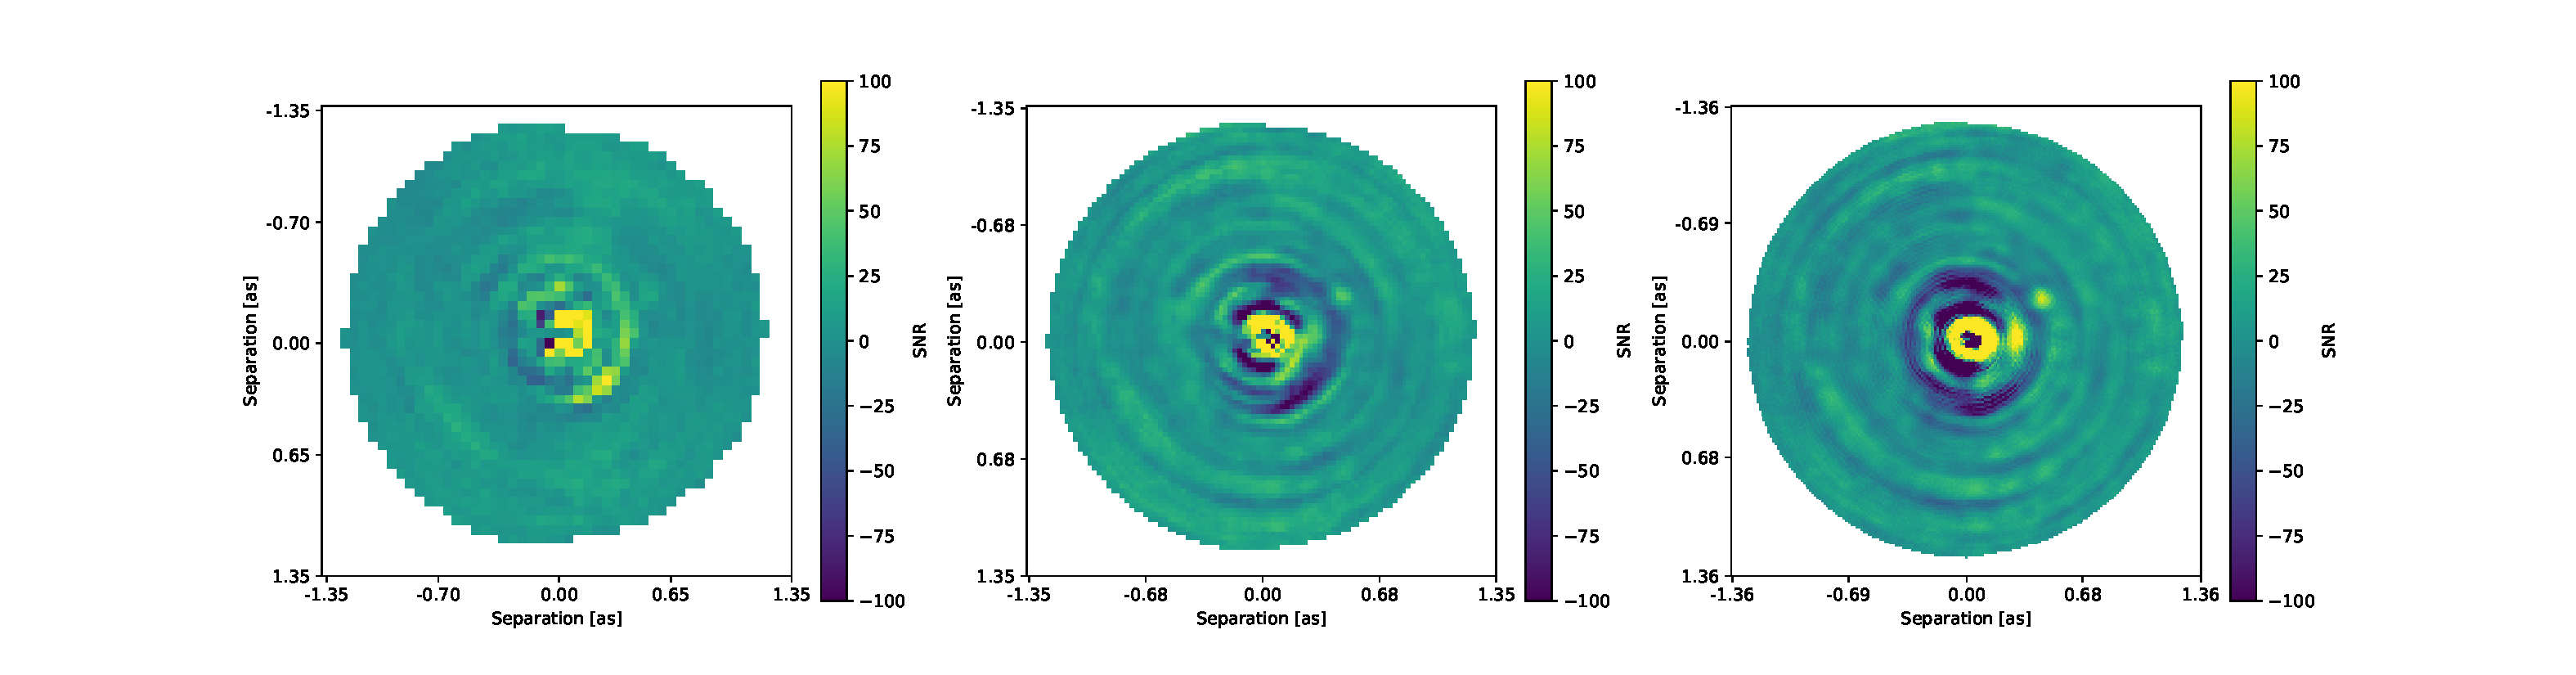
\includegraphics[width=1.25\linewidth]{scaling_3}
	\caption{\label{fig:SNROut} Typical example using $\beta$ Pic b of an output from PACO for different resolution scaling. Left is 0.5 times scaling, centre is 1.0, right is 2.0. The SNR increase as the scaling increases, as the template PSF is able to be positioned more accurately over the source.}
\end{figure}

\begin{figure}[h]
	%\includegraphics[width=\linewidth]{}
	\caption{\label{fig:FluxRetrieval} The iterative flux method is unbiased, and accurately retrieves the flux of an injected point source. The flux estimator is/isn't efficient, and provides greater/less precision than retrieval using negative source injection.}
\end{figure}
\subsection{Pynpoint Usage}
The PACO algorithm has been incorporated as a module into the Pynpoint analysis pipeline for exoplanet detection.
Pynpoint modules are added to a pipeline, with intermediate results stored in a local database.
Tutorials and examples can be found at \url{XXXXXXX}.

PACO can be run as a module following standard preprocessing of ADI data such as centering, cropping, dark frame subtraction etc.
It can be added to the pipeline using the function 
\begin{verbatim}
pynpoint.processing.PACOModule(...)
\end{verbatim}
The module contains many user-adjustable parameters as detailed below.
\begin{itemize}
	\item[] \verb|name_in|:
	\item[] \verb|image_in_tag|:
	\item[] \verb|psf_in_tag|:
	\item[] \verb|snr_out_tag|:
	\item[] \verb|flux_out_tag|:
	\item[] \verb|psf_rad|:
	\item[] \verb|scaling|:
	\item[] \verb|algorithm|:
	\item[] \verb|flux_calc|:
	\item[] \verb|threshold|:
	\item[] \verb|flux_prec|:
	\item[] \verb|verbose|:
\end{itemize}
The results (SNR maps, flux maps, point source coordinates and flux estimates) are stored in the Pynpoint database, and can be output using the standard Pynpoint IO functions.

PACO has also been added to Pynpoint's contrast curve module, where it can be selected as an option using the \verb|algorithm| argument. Additional parameters 

Runtime analysis: parallelized, but still basically unusable on large datasets.
\section{Results}
\subsection{Test Data}
\begin{figure}[h]
	\hspace{-3.5em}
	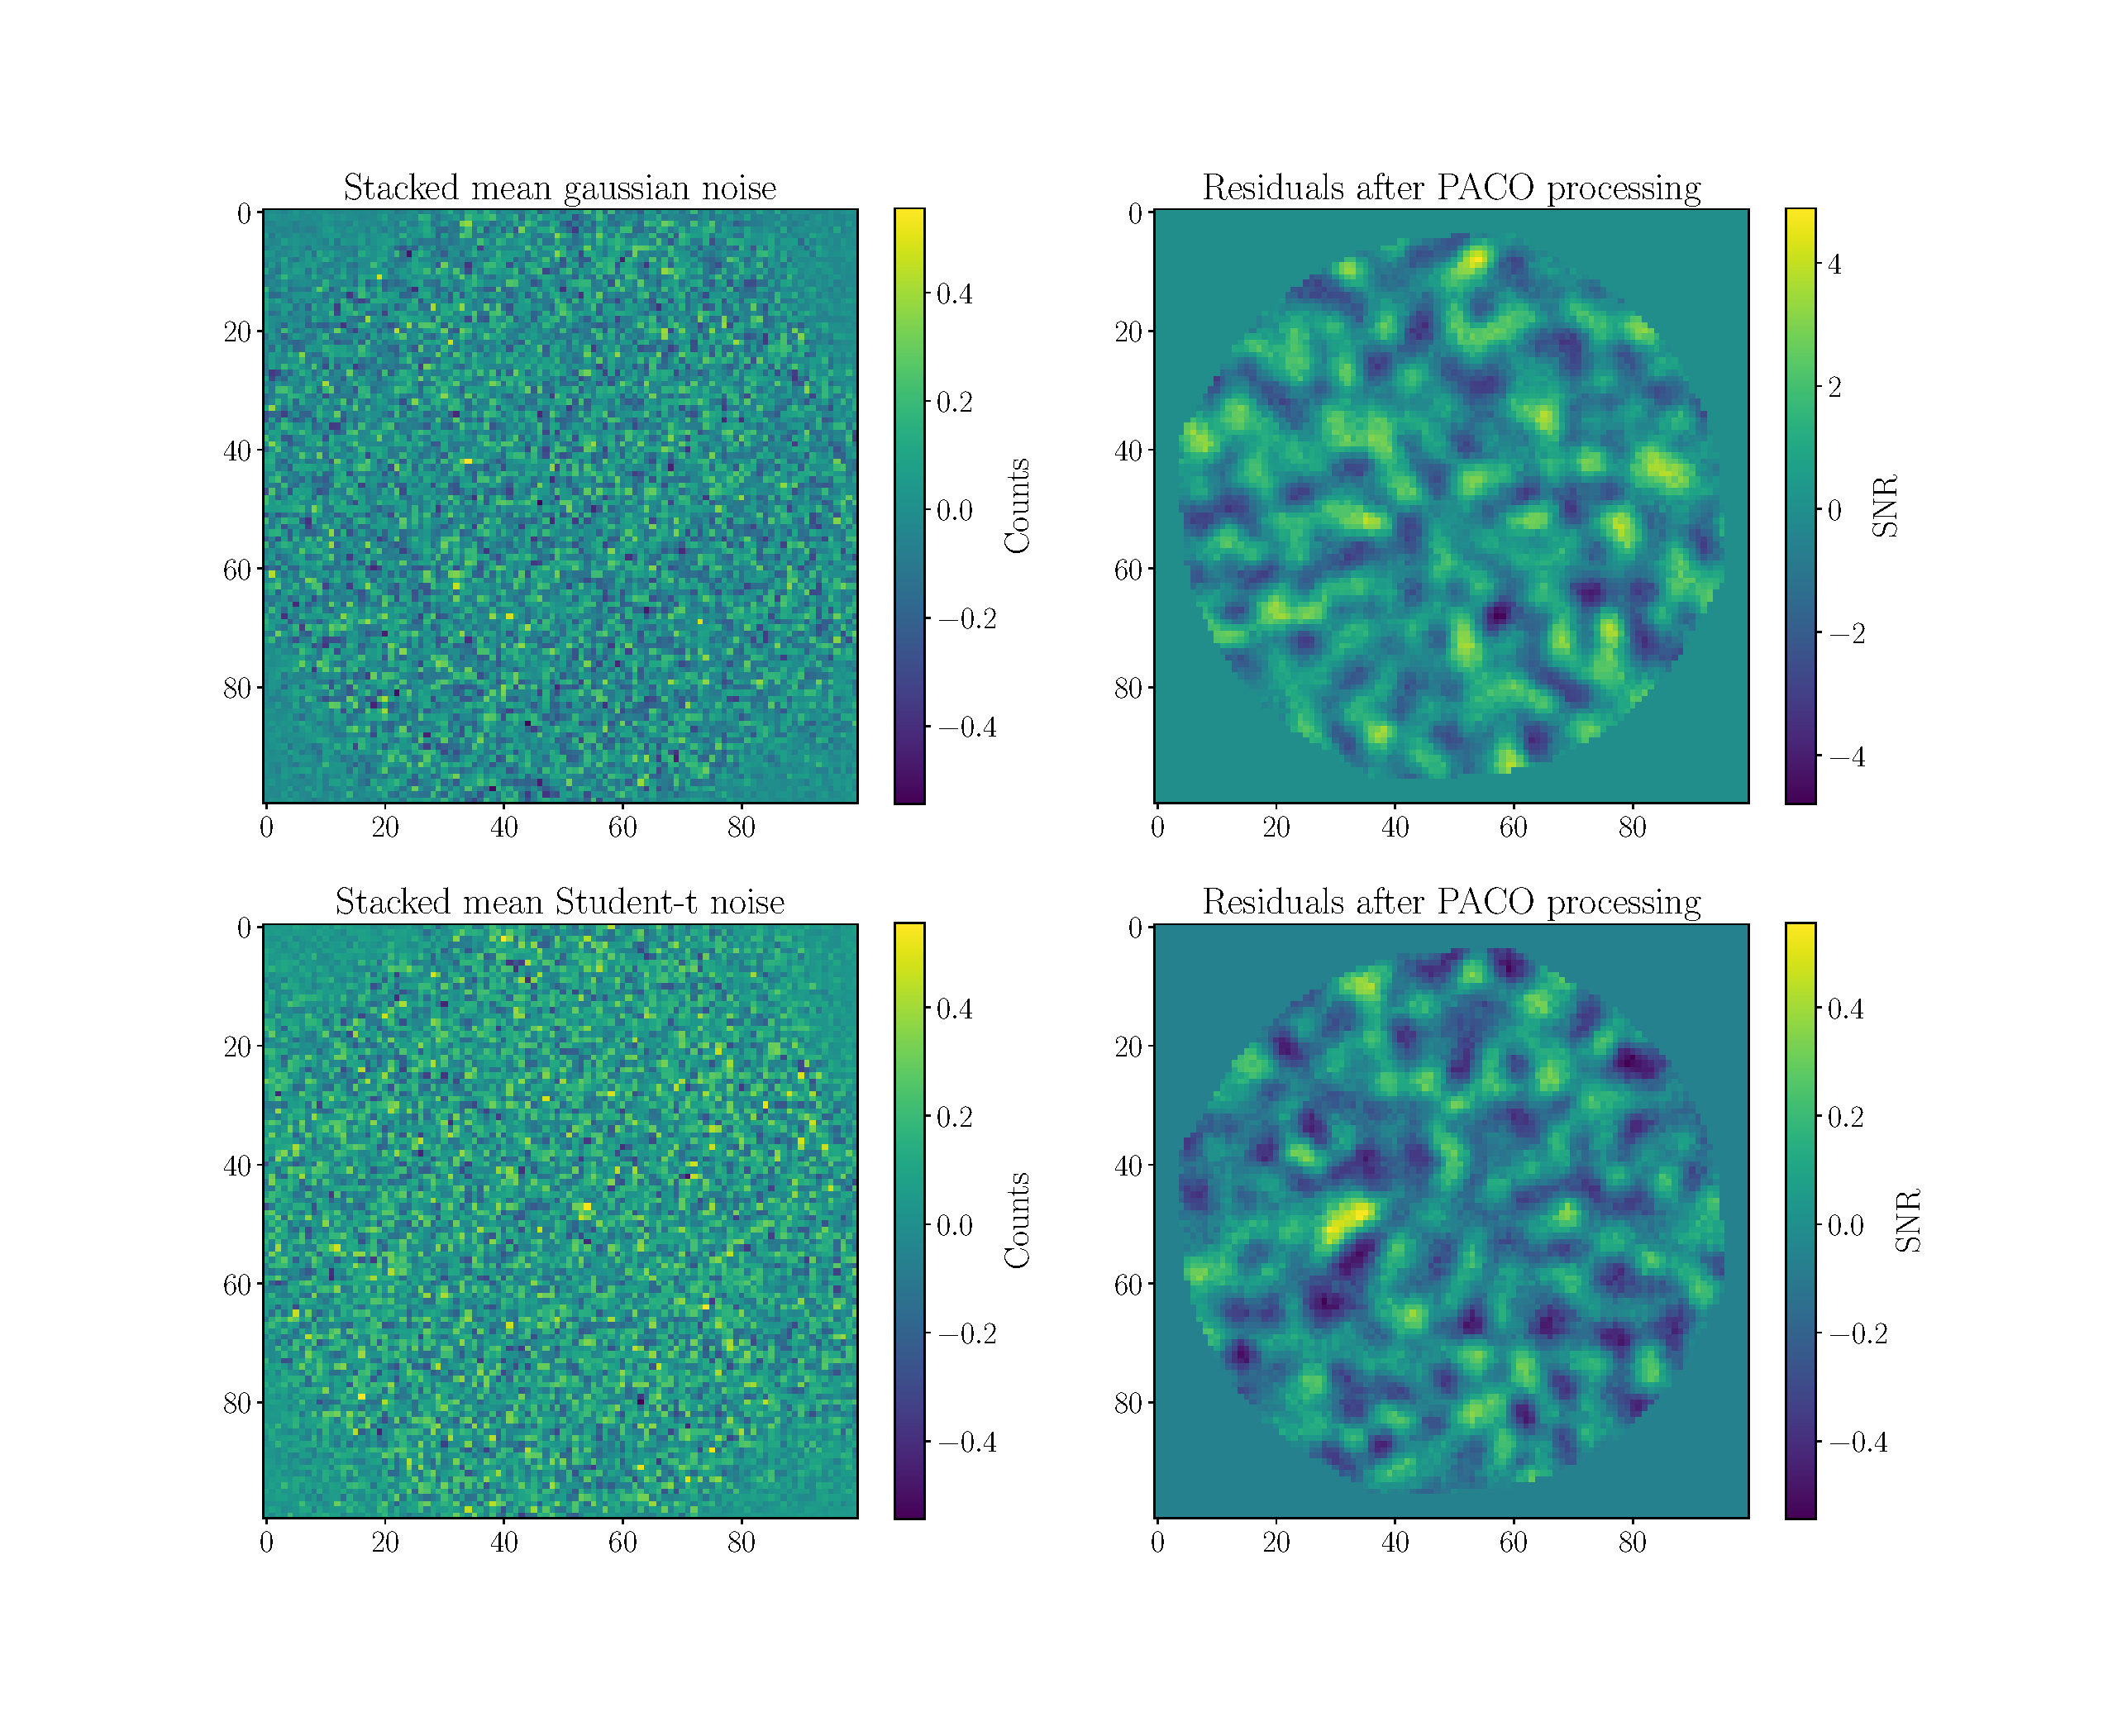
\includegraphics[width=1.25\linewidth]{beforeafter_3}
	\caption{\label{fig:noise} \textbf{Top}: On the left, random noise was drawn from a Gaussian distribution (mean 0, width 1), the shown image is the mean of the stacked and de-rotated image sequence. 
		The right image shows the residuals from processing the image sequence with PACO.
		\textbf{Bottom}: The same as above, but with noise drawn from a Student-t distribution (5 degrees of freedom). The magnitude of the SNR is lower due to the wider distribution of the background noise. (see Fig. \ref{fig:processed})}
\end{figure}
\begin{figure}[h]
	\centering
	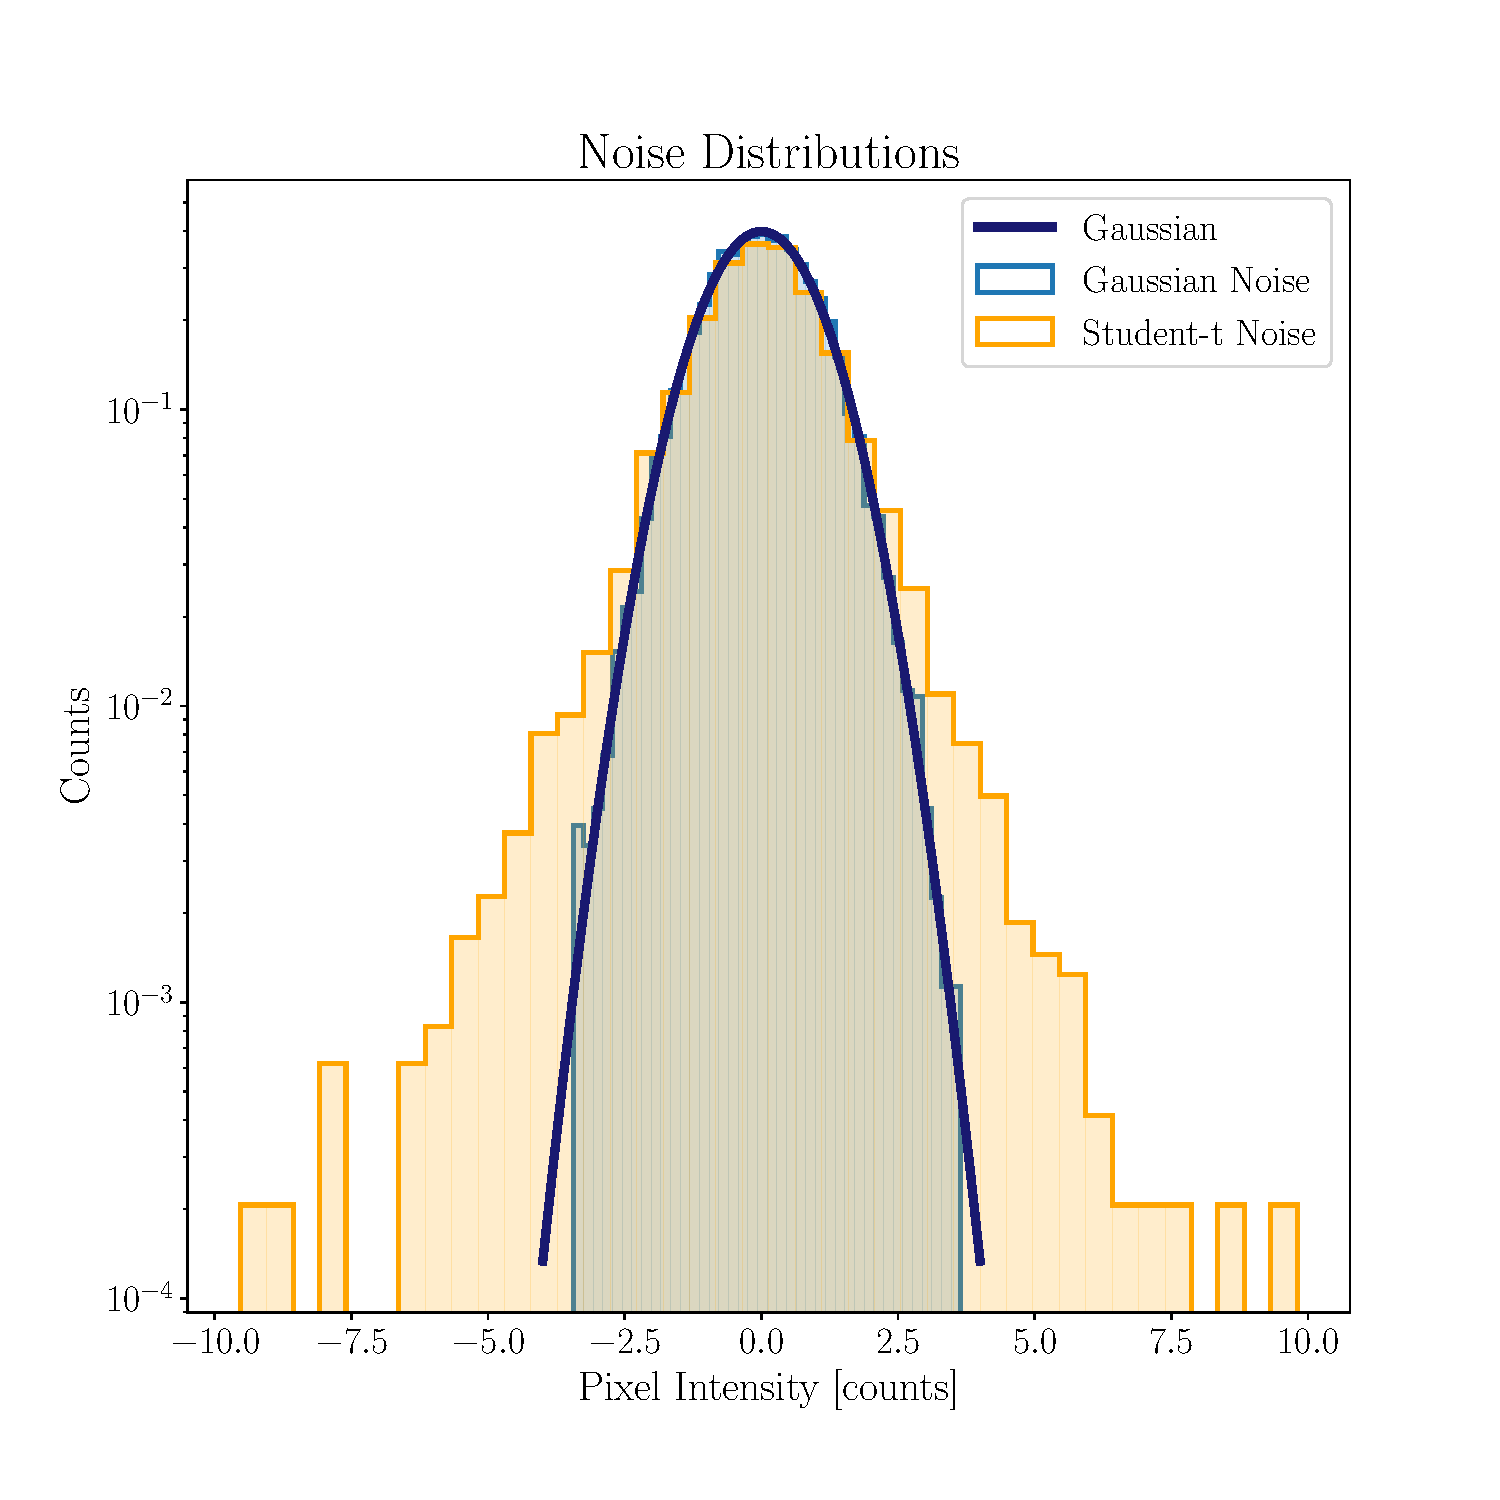
\includegraphics[width=\linewidth]{prepacostats}
	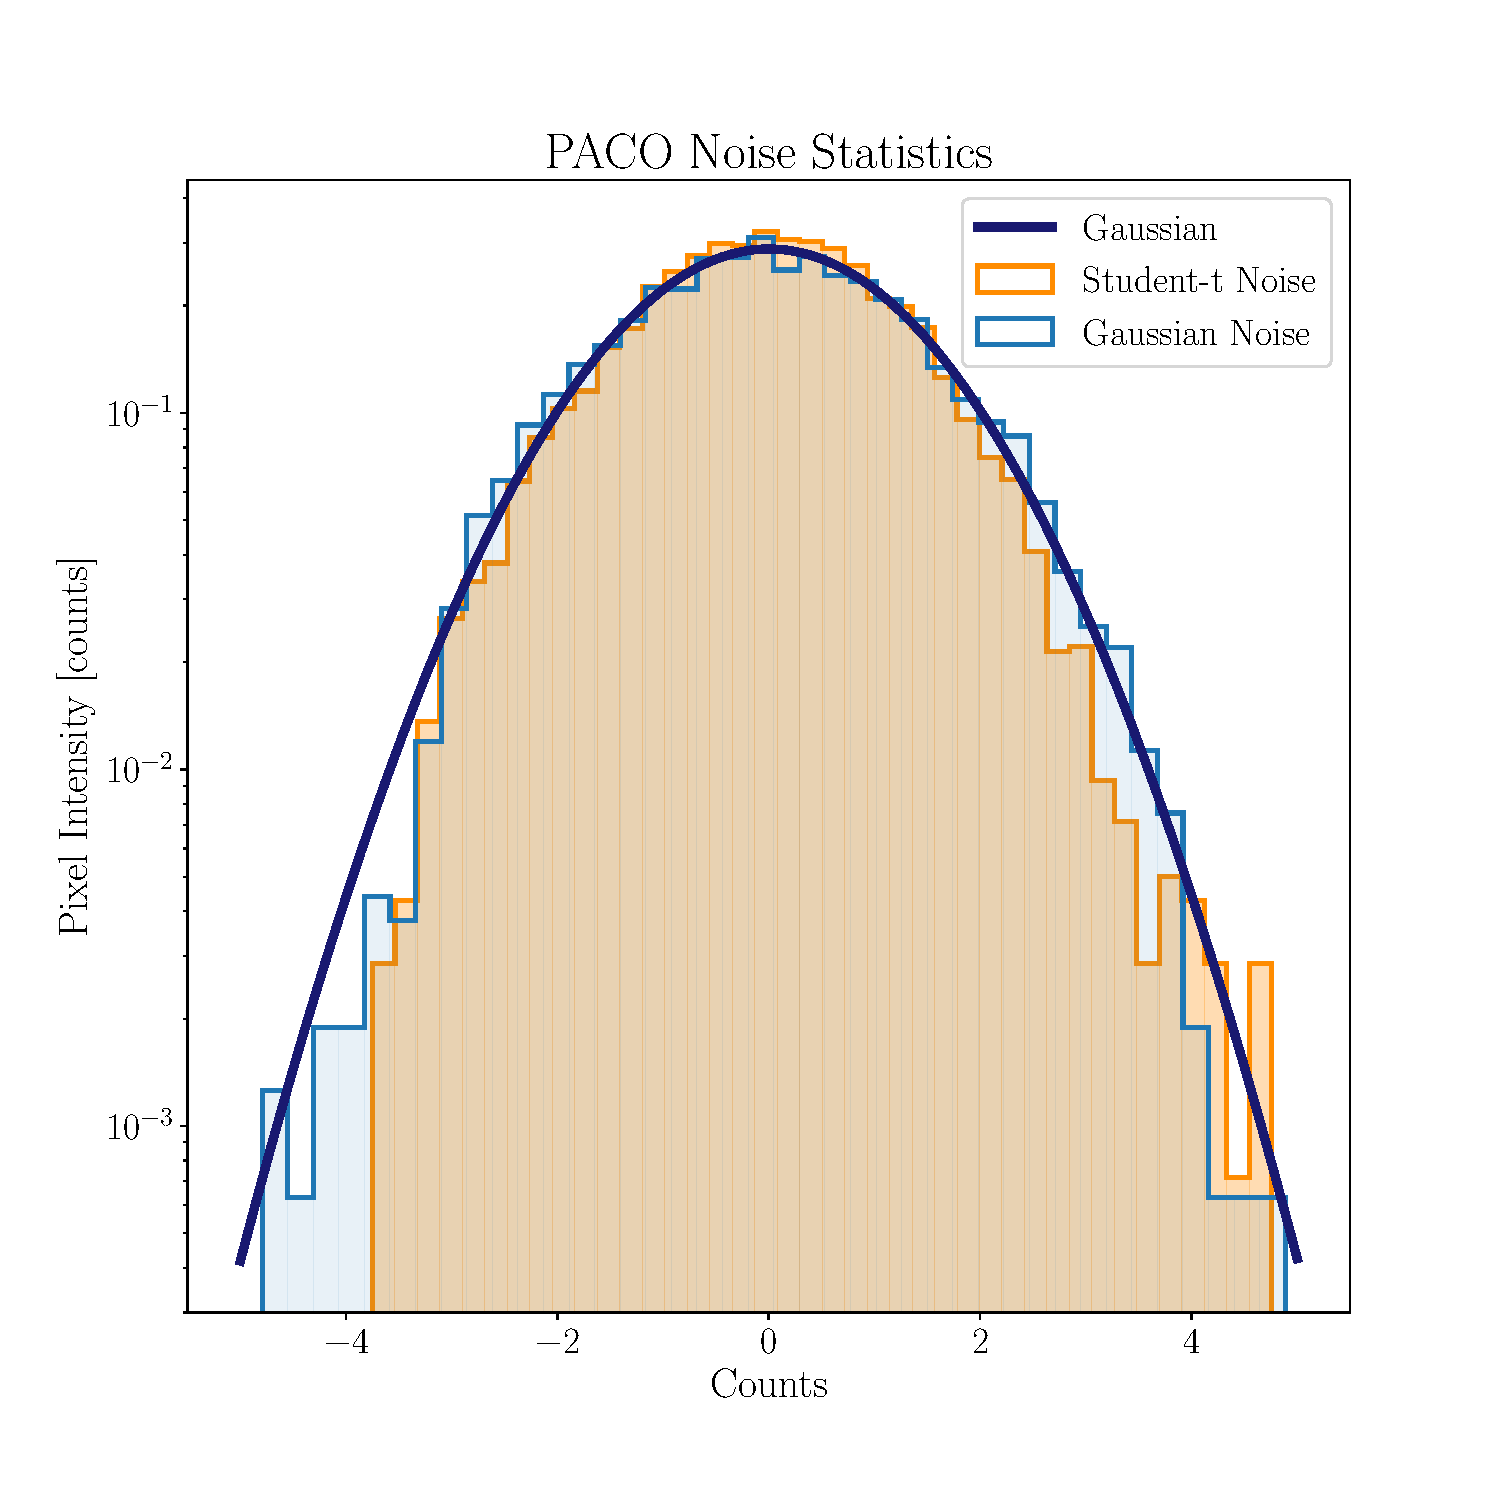
\includegraphics[width=\linewidth]{PACONoise}
	\caption{\label{fig:processed} Testing PACO on Gaussian and Student-t distributed noise. PACO residuals for both are Gaussian distributed.}
\end{figure}
\begin{figure}[h]
	\hspace{-2.5em}
	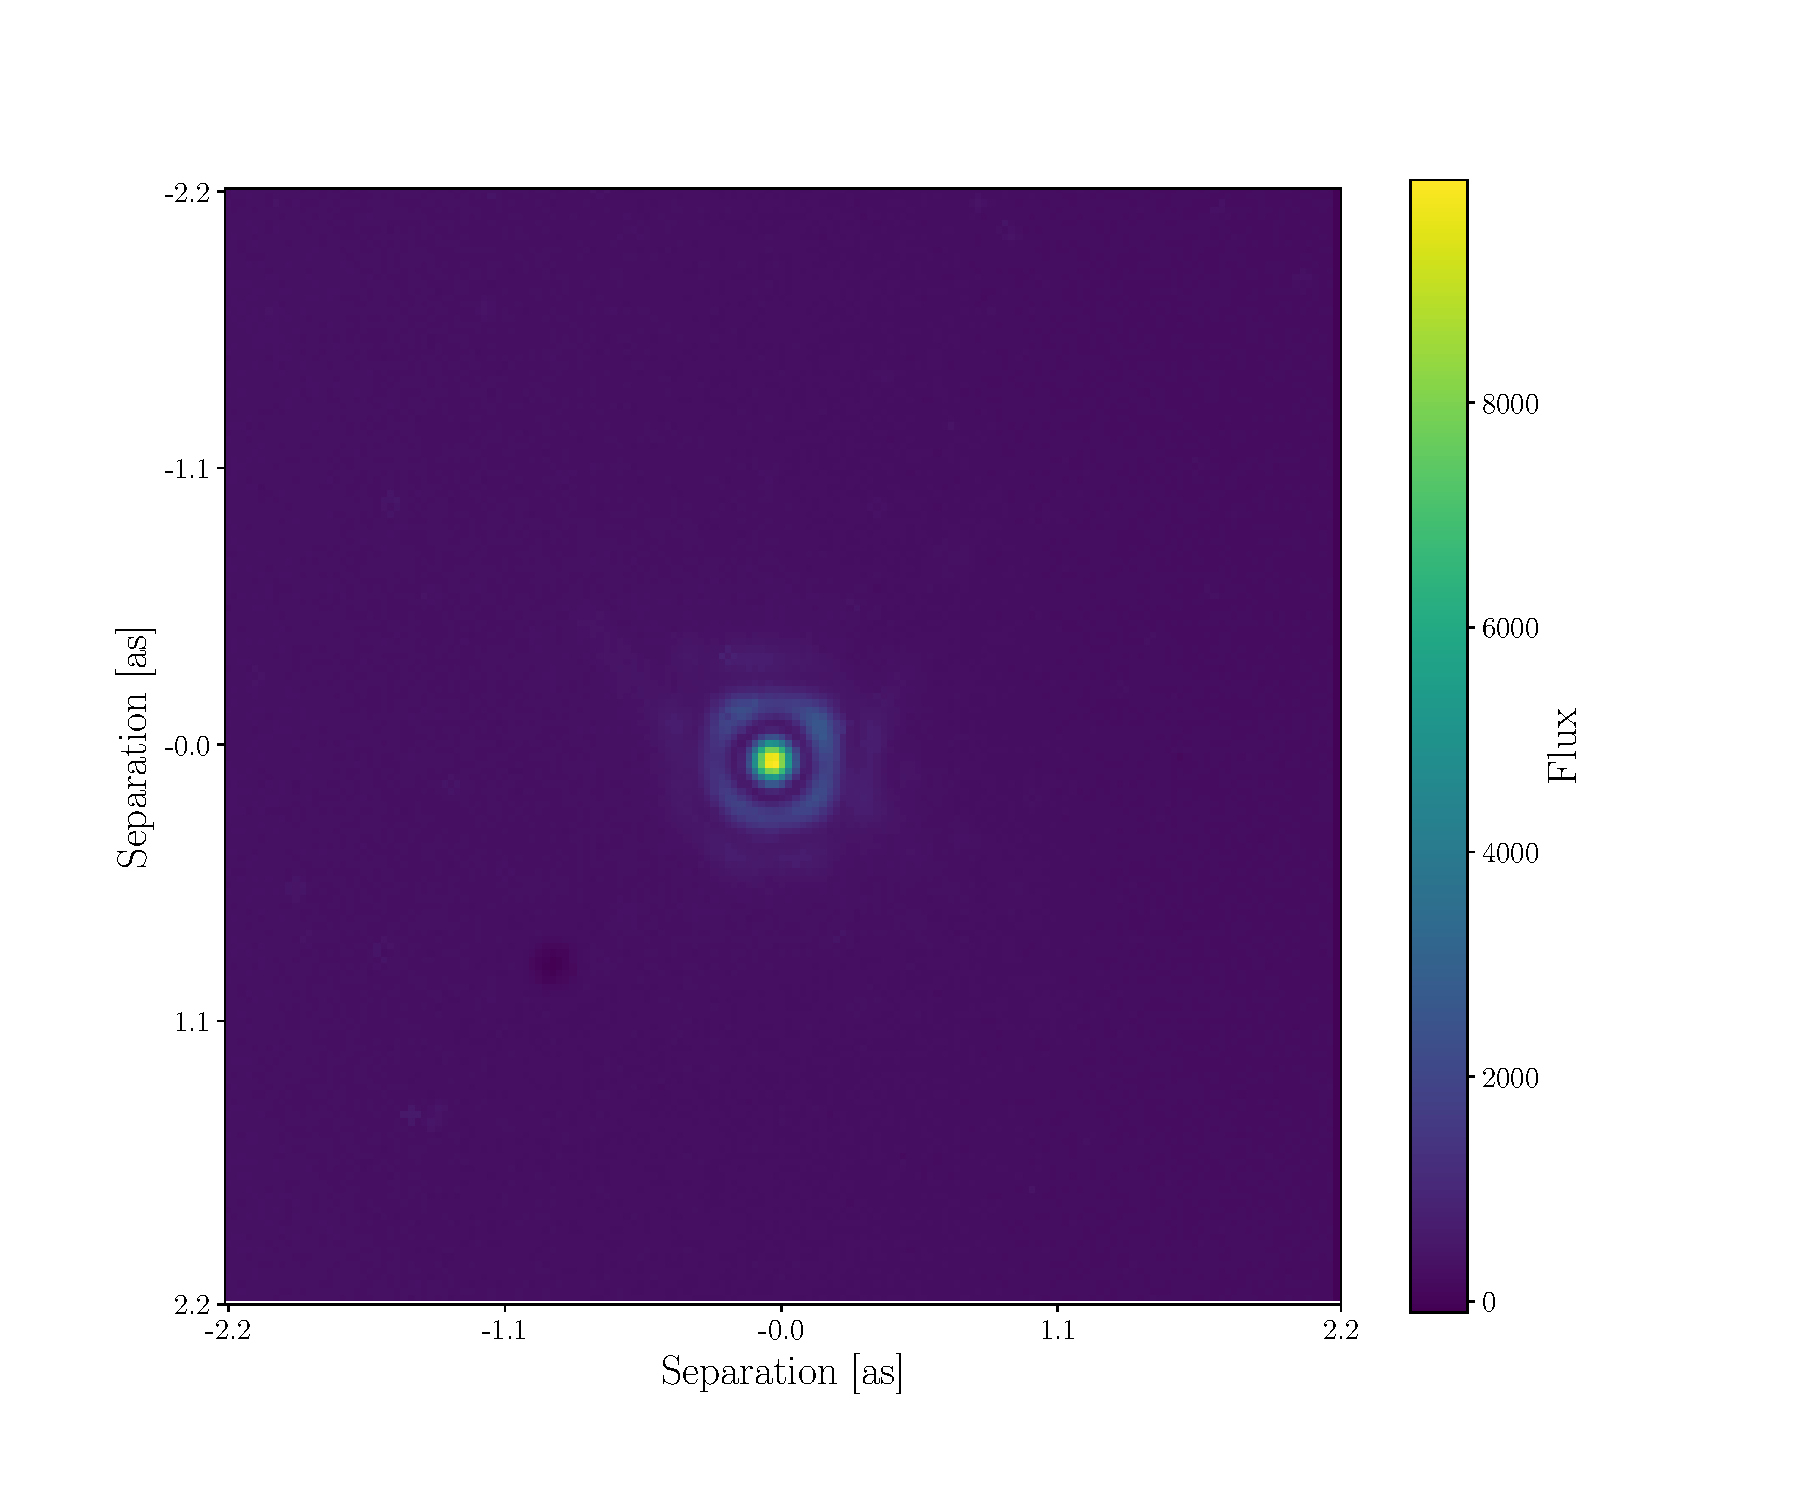
\includegraphics[width=1.25\linewidth]{HD131399}
	\caption{\label{fig:TestData} Example of single frame from HD131399 dataset used for testing.}
	 %Position of injected sources are marked in XXX, while position of 5$\sigma$ detections are marked in YYY.}
\end{figure}

\subsection{Statistics}

\begin{figure}[h]
	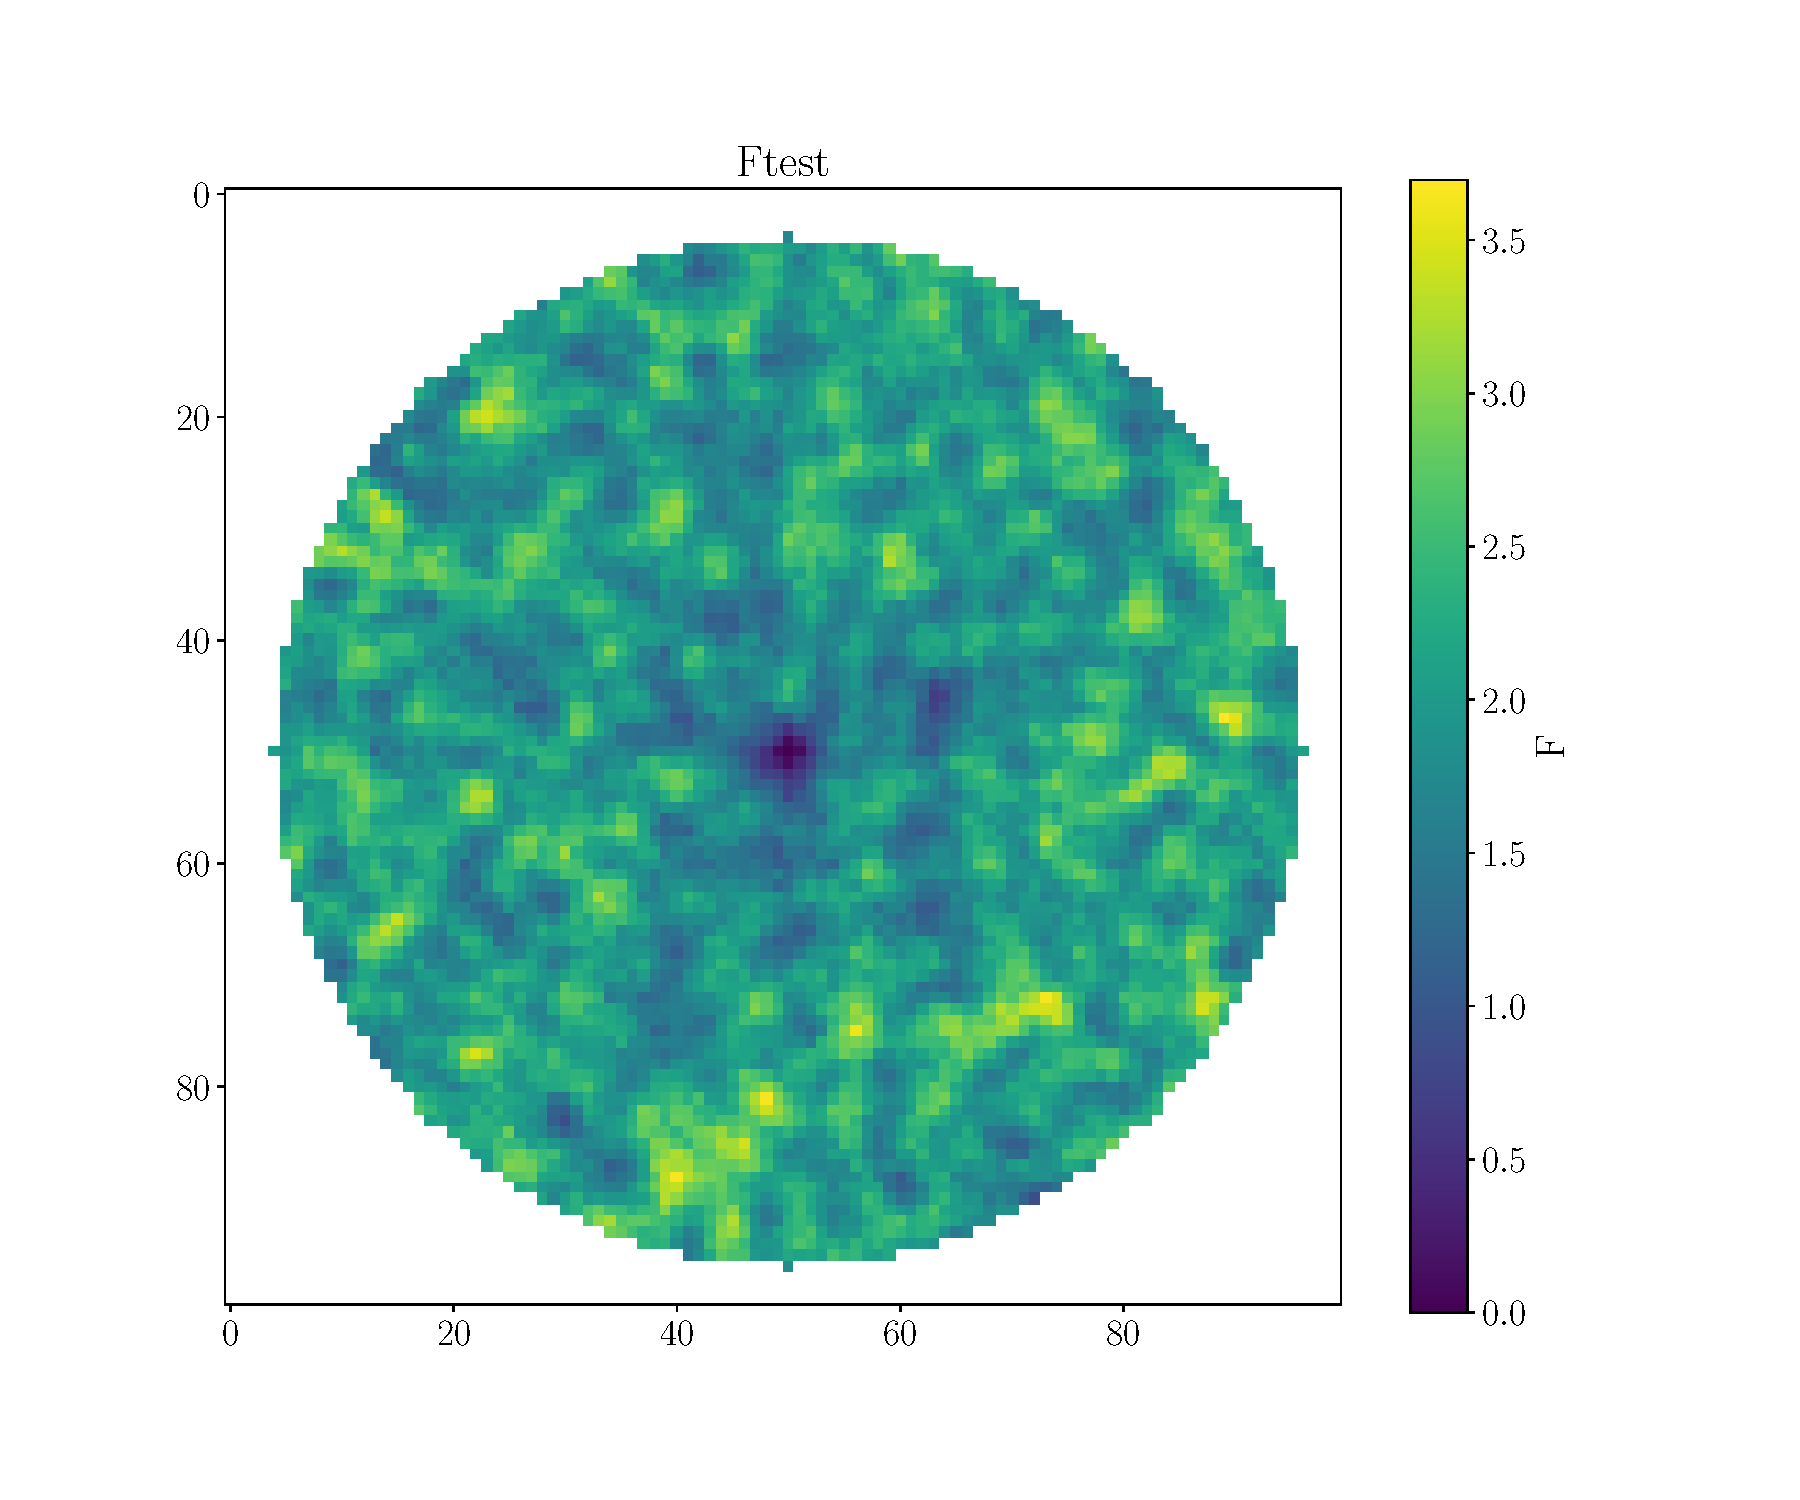
\includegraphics[width=1.1\linewidth]{Ftest}
	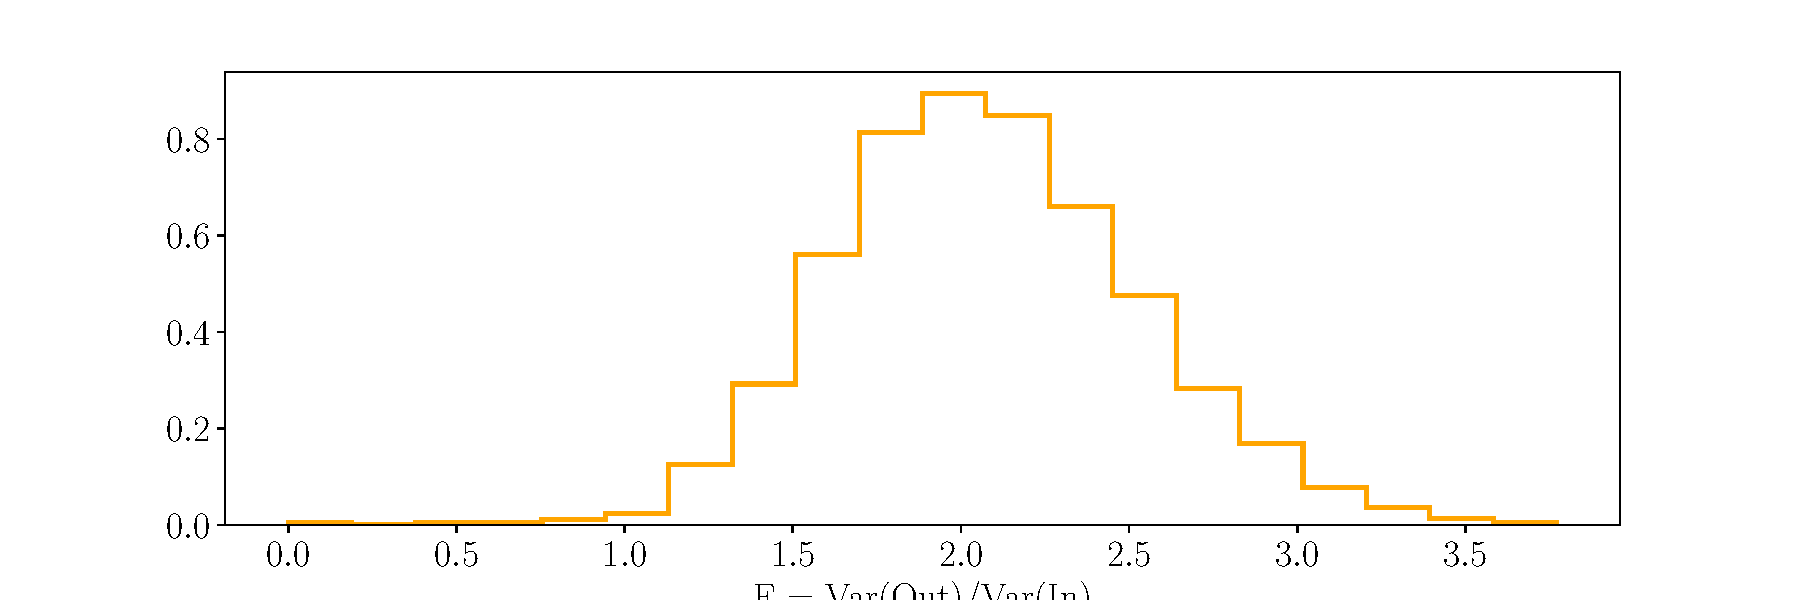
\includegraphics[width=\linewidth]{Ftestdist}	
	\caption{\label{fig:Anova} Here we show that the estimator for the variance of the flux accurately is a good estimator.}
\end{figure}
\begin{figure}[h]
	%\includegraphics[width=\linewidth]{}
	\caption{\label{fig:Contrast} We can compute a contrast curve for a given dataset, either using standard aperture masking, or by using PACOs flux retrieval. This is compared with a contrast curve from Pynpoints PCA model on the same dataset for reference.}
\end{figure}
\begin{figure}[h]
	%\includegraphics[width=\linewidth]{}
	\caption{\label{fig:Completeness} For sources injected at XXX sigma, PACO accurately retrieves YY\% of the sources at the same significance.}
\end{figure}
\begin{figure}[h]
	%\includegraphics[width=\linewidth]{}
	\caption{\label{fig:ROC} We can also compare the true positive fraction against the false positive fraction using an ROC curve.}
\end{figure}
\section{Comparisons}
% Compare to original paper
% Compare to other algorithms? If time permitting
\section{Discussion}
%Spectral PACO, datasets,
\section{Conclusions}
\section*{Acknowledgments}
Sascha Quanz, Tomas Stolker, Anna Boehle, Tim ????, Natalia ???, O. Flasseur, ???? and ???? for writing the original algorithm
\bibpunct{(}{)}{;}{a}{}{,} % to follow the A&A style
\bibliographystyle{aasjournal}
\bibliography{paco_bib.bib}

\end{document}
